% !TEX program = xelatex
% 中文论文基础模板（ctexart），使用 XeLaTeX 编译
\documentclass[UTF8,12pt,a4paper]{ctexart}

% ---------- 宏包 ----------
\usepackage[margin=25mm]{geometry}   % 页边距（版心宽度 160mm）
\usepackage{graphicx}                % 插图
\usepackage{booktabs}                % 三线表
\usepackage{longtable}               % 跨页长表
\usepackage{array}                   % 表格列宽控制
\usepackage{amsmath,amssymb}         % 数学公式
\usepackage{caption}                 % 图表标题
\captionsetup{font=small,labelfont=bf,labelsep=quad,skip=6pt}
\usepackage{needspace}
\setlength{\parindent}{2em}
\setlength{\parskip}{0pt}
\linespread{1.30}
\setlength{\emergencystretch}{2em}
\raggedbottom
\setlength{\textfloatsep}{12pt plus 2pt minus 2pt}
\setlength{\intextsep}{10pt plus 2pt minus 2pt}
\setlength{\floatsep}{10pt plus 2pt minus 2pt}
\setlength{\LTpre}{8pt}
\setlength{\LTpost}{9pt}
\setlength{\LTcapwidth}{\textwidth}
\setcounter{topnumber}{2}
\renewcommand{\topfraction}{0.85}
\renewcommand{\textfraction}{0.12}
\renewcommand{\floatpagefraction}{0.65}
\widowpenalty=10000
\clubpenalty=10000
\usepackage[hidelinks]{hyperref}     % 超链接（放最后）

% ---------- 所有标题左对齐 ----------
\ctexset{
  section/format = \zihao{4}\heiti\raggedright,
  section/beforeskip = 14pt,
  section/afterskip = 7pt,
  subsection/format = \zihao{-4}\heiti\raggedright,
  subsection/beforeskip = 10pt,
  subsection/afterskip = 4pt,
  subsubsection/format = \normalsize\heiti\raggedright
}

% ---------- 标题编号：一、 / 1.1 / 1.1.1 ----------
\ctexset{section = {name = {,、}, number = \chinese{section}}}
\renewcommand{\thesubsection}{\arabic{section}.\arabic{subsection}}
\renewcommand{\thesubsubsection}{\arabic{section}.\arabic{subsection}.\arabic{subsubsection}}

\newcolumntype{L}[1]{>{\raggedright\arraybackslash}p{#1}}
\newcolumntype{C}[1]{>{\centering\arraybackslash}p{#1}}
\newcolumntype{R}[1]{>{\raggedleft\arraybackslash}p{#1}}

% ---------- 摘要与正文等宽 ----------
\renewenvironment{abstract}{%
  \par\vspace{4pt}%
  {\centering\zihao{-4}\heiti \abstractname\par}%
  \vspace{9pt}\linespread{1}\fontsize{12pt}{21pt}\selectfont\par%
}{%
  \par\vspace{8pt}%
}

% ---------- 标题信息 ----------
\newcommand{\papertitle}{CogniVista 观睿\\[5pt]大学本科生全域认知智能赋能平台\\[7pt]全生命周期工程管理报告}

\begin{document}
\pagestyle{plain} % 页码在页脚居中，无页眉

% 居中的标题
{\centering\fontsize{18pt}{25pt}\selectfont\heiti \papertitle\par}
\vspace{10pt}

% ---------- 摘要与关键词 ----------
\begin{abstract}
这份报告站在项目经理的位置，记录 CogniVista 观睿平台——一个总投资 1 亿元、周期 36 个月的项目——从立项、规划、建设，再到试点、推广与后评价的各项管理安排。平台面向跨专业本科生，靠跨学科概念图谱、思辨对话和决策沙盘来辅助学习。技术层面放弃底层模型的自主训练，把外部模型接口、12 个学科的知识库和交互工作台组合起来，资金主要投向能长期使用的知识资源和教学功能。

范围与进度方面，报告用工作分解结构把交付边界说清楚，将知识库、模型网关、前端交互与安全测评拆成一项项可验收的任务，建设顺序则交给关键路径和阶段里程碑来约束。成本管理以 1 亿元总投资为上限，划出 9,000 万元直接工程成本、600 万元应急储备和 400 万元管理储备，凑成 9,600 万元的成本基准。预算同时套用参数估算、自下而上估算和类比估算三种办法，再对照季度资金计划看花钱的快慢。

针对第 18 个月的模拟执行情景，报告借用计划值、挣值和实际成本三组数字，看出 300 万元的成本超支和 400 万元的进度偏差，进而拆解知识库清洗返工与前端性能不足带来的影响，给出自动化解析、缓存优化和人员支援几条办法，并借助完工估算去判断预算有没有被突破。质量与安全管理把响应速度、检索质量、内容溯源、隐私保护以及上线验收逐项列成检查要求；资源与风险管理这边，则靠责任矩阵、风险登记册和期望损失测算，把负责人和储备动用条件定下来。

后评价阶段要重点核对交付范围、工期、决算和服务效果，同时把学生能力有没有提升，与访问量、注册人数这类指标分开来看。需要说明的是，本文只是课程模拟案例，预算单价、风险概率和执行结果都用来演示管理方法，并不代表已经落地的真实成果；真要实施，还得按调研、采购报价和试点测评重新校一遍。
\end{abstract}

{\fontsize{10.5pt}{17pt}\selectfont\noindent\textbf{关键词：}工程管理；全生命周期；成本控制；混合检索增强；挣值分析；项目后评价\par}
\clearpage

% ---------- 正文 ----------
\section{项目概况与全生命周期安排}

\subsection{建设背景与技术路线选择}
把 AI 用在高等教育里，得同时照顾学习支持和教育伦理两条线\textsuperscript{[1-2]}。本项目打算投入 1 亿元，建一个跨学科的认知辅助平台，帮本科生核验论证依据、比较学业与生涯选项，重心放在辅助独立判断上，而不是替他们跳过推理这一步。

选技术路线时，采购、运维、升级乃至退出的成本要一并盘算。自建通用大模型意味着硬件和训练人员都得长期养着，所以本方案不碰底层模型的自训，把资金转到知识资源、教学交互和接口服务上，固定资产投入和技术替换成本都能压下来。

算力层按任务难易调度对话模型或推理模型\textsuperscript{[3]}，语义缓存用来砍掉重复请求；知识库覆盖 12 个学科门类，套用检索增强生成\textsuperscript{[4]}，回答里会带上可核对的出处。交互层放概念图谱（图~\ref{fig:lens_galaxy}）、思辨对话、决策沙盘和认知档案。这些图只是原型示意，不能拿来当规模化性能的验收凭证。

\begin{figure}[!htb]
    \centering
    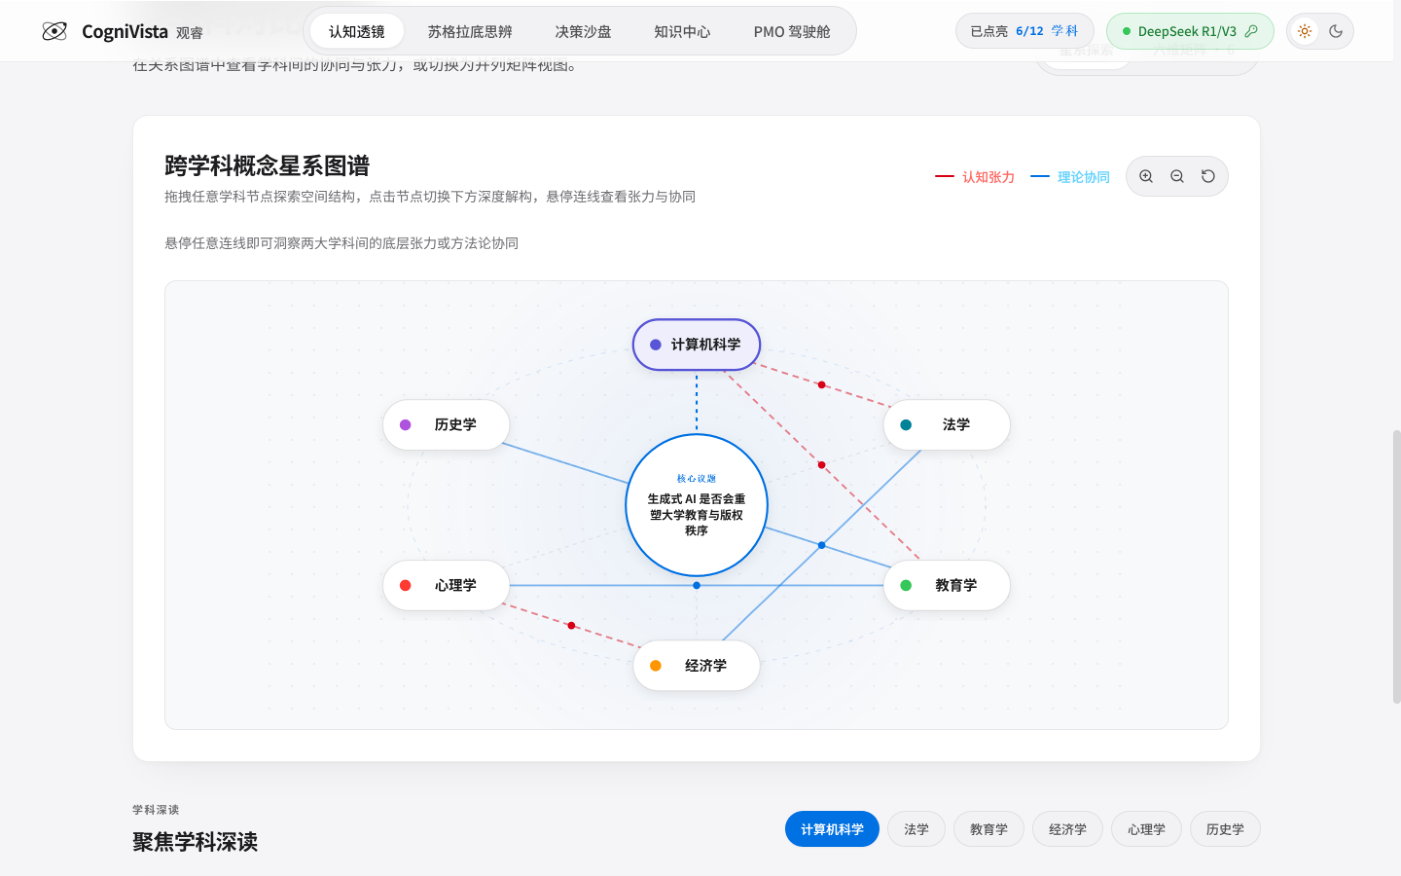
\includegraphics[width=0.82\linewidth,height=0.30\textheight,keepaspectratio]{figures/fig_01_lens_galaxy.png}
    \caption{CogniVista 观睿原型系统：全域跨学科认知透镜与概念星系图谱}
    \label{fig:lens_galaxy}
\end{figure}

\subsection{全生命周期五阶段划分与《项目章程》}
项目总周期 36 个月（2026 年 9 月至 2029 年 8 月），按管理任务切成五段。第 1—3 个月是启动立项，把需求调研、可行性研究、资金批复和项目章程做完；第 4—6 个月是规划与原型，冻结范围、进度、成本三项基准，并确认原型、采购首批文献。第 7—21 个月是核心建设，算力、文献入库和前后端研发并行推进，第 18 个月做一次中期挣值检查；第 22—24 个月转入测评试点，完成安全测评后在 10 所高校公测；最后第 25—36 个月是推广收尾，处理高校推广、运营交接和项目后评价。

《项目章程》把预算、采购和进度协调的权限交给项目经理，统管 75 名专职人员和 120 名学科顾问。管理储备要经发起人审批才能动用，交付与验收的指标列在表~\ref{tab:wbs}《工作分解与验收基准》里，范围不能随便扩，成本基准也不能随意破。

\section{项目范围与时间管理}

\subsection{范围界定、工作分解与变更控制}
需求阶段打算用学生问卷加教师访谈，把教学诉求翻译成可测试的指标，落到《需求跟踪矩阵（RTM）》里。范围说明书圈进了 12 学科知识库、模型网关、交互工作台、安全测评和高校推广，底层模型自训、既有教务系统改造、论文代写这三样明确排除在外。每一条需求都配好责任人、交付物和验收方法，免得新功能冒出来挤占既定预算。

工作分解结构铺满管理推广、算力、知识库、后端、前端和质量安全六类工作，跟成本科目一一对应；应急储备单独拎出来，不当工程交付物（表~\ref{tab:wbs}）。M6、M12、M18、M24、M36 这几个节点，都要对着 RTM 逐项核验并签字留档。基准冻结以后再冒出来的需求，得先交变更申请，由变更控制委员会（CCB）估完工期和预算影响再定收不收。

\begingroup
\linespread{1}\fontsize{9.8pt}{12.5pt}\selectfont\songti
\setlength{\tabcolsep}{4pt}
\renewcommand{\arraystretch}{1.20}
\begin{longtable}{@{}L{3.15cm}L{4.95cm}L{5.25cm}R{1.80cm}@{}}
\caption{工作分解与验收基准\label{tab:wbs}} \\
\toprule[0.8pt]
\textbf{工作项目} & \textbf{具体任务} & \textbf{交付与验收标准} & \textbf{预算/万元} \\
\midrule[0.5pt]
\endfirsthead
\multicolumn{4}{@{}l@{}}{\linespread{1}\fontsize{9.8pt}{12.5pt}\selectfont\songti （续表）工作分解与验收基准} \\
\toprule[0.8pt]
\textbf{工作项目} & \textbf{具体任务} & \textbf{交付与验收标准} & \textbf{预算/万元} \\
\midrule[0.5pt]
\endhead
\bottomrule[0.8pt]
\endfoot
\bottomrule[0.8pt]
\endlastfoot
项目管理与推广 & 项目治理与审计；高校推广与思辨大赛；驻场运维 & 覆盖不少于 100 所高校、100 万学生，完成三届思辨大赛 & 800.00 \\
算力与网关 & 模型接口服务；本地向量与微调集群；语义缓存与灾备 & 日均 50 万次调用目标；缓存命中率不低于 35\% & 2,200.00 \\
学科知识库 & 文献版权采购；多模态解析清洗；专家思辨图谱标注 & 500 万份文献、15 万条标注；召回率不低于 90\% & 2,600.00 \\
后端研发 & 双模型路由；混合检索溯源；高校认证对接 & 首字响应不超过 1.2 秒；回答附带原文出处 & 1,400.00 \\
前端研发 & 跨学科概念透镜；思辨对话；决策沙盘与多端适配 & 兼容网页、移动端与大屏；目标设备帧率不低于 30fps & 1,400.00 \\
质量与安全 & 防幻觉与防代写；安全测评与压测；安全审计 & 幻觉率不高于 1.5\%；完成安全测评及整改 & 600.00 \\
应急储备 & 已识别风险的初始储备，纳入成本基准 & 按期望损失测算，审批后转入风险任务预算 & 600.00 \\
\midrule[0.4pt]
\textbf{成本基准（BAC）} & \textbf{不含 400 万元管理储备} & \textbf{工作范围与预算科目相互对应} & \textbf{9,600.00} \\
\end{longtable}
\endgroup

\subsection{关键路径排期与里程碑控制}
核心活动走计划评审技术（PERT）的三点估算，用期望工期 $t_e=(O+4M+P)/6$ 和标准差 $\sigma=(P-O)/6$ 来算持续时间，再靠关键路径法推出总工期和各活动的浮动时间（表~\ref{tab:schedule}）。关键路径是“立项调研$\rightarrow$规划与原型$\rightarrow$文献清洗入库$\rightarrow$联调压测$\rightarrow$测评试点$\rightarrow$推广后评价”，总期望工期 36 个月。真要排期，还得再看看资源冲突和外部审批的等待时间。

\begingroup
\linespread{1}\fontsize{9.8pt}{12.5pt}\selectfont\songti
\setlength{\tabcolsep}{4pt}
\renewcommand{\arraystretch}{1.20}
\begin{longtable}{@{}L{3.90cm}C{2.70cm}C{1.65cm}C{1.90cm}L{4.72cm}@{}}
\caption{核心活动工期与里程碑\label{tab:schedule}} \\
\toprule[0.8pt]
\textbf{核心活动名称} & \textbf{O/M/P（月）} & \textbf{期望工期} & \textbf{总浮动} & \textbf{里程碑节点} \\
\midrule[0.5pt]
\endfirsthead
\multicolumn{5}{@{}l@{}}{\linespread{1}\fontsize{9.8pt}{12.5pt}\selectfont\songti （续表）核心活动工期与里程碑} \\
\toprule[0.8pt]
\textbf{核心活动名称} & \textbf{O/M/P（月）} & \textbf{期望工期} & \textbf{总浮动} & \textbf{里程碑节点} \\
\midrule[0.5pt]
\endhead
\bottomrule[0.8pt]
\endfoot
\bottomrule[0.8pt]
\endlastfoot
立项调研与章程签署 & 2.5/3.0/3.5 & 3.0 & 0（关键） & 第 3 月：立项批复 \\
规划基准与原型封版 & 2.5/3.0/3.5 & 3.0 & 0（关键） & 第 6 月：基准冻结 \\
算力上架与网关研发 & 5.0/6.0/8.0 & 6.2 & 5.8 & 支撑第 12 月分批入库 \\
12 学科文献清洗入库 & 10.0/12.0/14.0 & 12.0 & 0（关键） & 第 12/18 月：分批入库 \\
智能体与前端并行研发 & 9.0/11.0/13.0 & 11.0 & 1.0 & 第 18 月：中期核查 \\
系统联调与压力测试 & 2.5/3.0/3.5 & 3.0 & 0（关键） & 第 21 月：预投产评审 \\
安全测评与十校公测 & 2.5/3.0/3.5 & 3.0 & 0（关键） & 第 24 月：公测验收 \\
百校推广与后评价 & 11.0/12.0/13.0 & 12.0 & 0（关键） & 第 36 月：决算后评价 \\
\end{longtable}
\endgroup

进度控制要盯紧两处：一是文献清洗，一点浮动时间都没有；二是前端研发，只剩一个月浮动。前后端照着约定好的接口并行开发，减少串行等待；交付进度按双周迭代对账，中期评审前先把人员支援和任务调整的预案备好。

\section{项目成本管理}

\subsection{1 亿元投资配置思路与估算方法}
1 亿元的总投资是这样分的：算力与网关 2,200 万元，学科知识库 2,600 万元，前后端研发合起来 2,800 万元，质量安全 600 万元，项目管理与推广 800 万元，加起来正好 9,000 万元直接工程成本。另外单列 600 万元应急储备，凑成 9,600 万元成本基准；还有 400 万元管理储备不进基准，动用要发起人点头。正式立项时，资金来源和适用的采购制度也得一并说清。

要避免成本估低了，工作量、单价和风险假设都得再核一遍\textsuperscript{[5]}。先看参数估算这条：100 万用户、15\% 日活、人均每天 3.3 次请求，一天下来约 49.5 万次请求；每次折成 4,000 个 Token，三年按 1,000 个等效满负荷服务日算，总共 1.98 万亿个 Token，缓存砍掉 35\% 后约剩 1.287 万亿个。接口资源包和通道费暂时列 1,100 万元，这是课程估值，不是供应商报价。500 万份文献按平均 16 页折算成 8,000 万页，解析与切片按 0.10 元/页估，得 800 万元。自下而上的算法呢：前端 25 人 $\times$ 24 月 $\times$ 1.75 万元/人月，是 1,050 万元；后端 25 人 $\times$ 24 月 $\times$ 1.90 万元/人月，是 1,140 万元；适配与认证按 15 人 $\times$ 18 月、均价约 2.26 万元/人月，取整列 610 万元，研发这一块合计 2,800 万元。类比估算则把版权采购暂列 1,200 万元、安全测评与审计 280 万元，动手前再用可比合同和报价校准。储备这块，按本例 592 万元的期望损失，初始预留 600 万元应急储备，总投资另留 400 万元管理储备。所有费用统一按含税口径，人月是综合成本，不会和采购科目重复计费。

\subsection{成本分解与资金使用基准}
预算照着表~\ref{tab:wbs} 的工作项目归集，明细落在表~\ref{tab:cbs}《成本分解与预算明细》里。多端适配与认证的费用按任务摊到前端和后端头上，省得重复计费。

\begingroup
\linespread{1}\fontsize{9.5pt}{12pt}\selectfont\songti
\setlength{\tabcolsep}{4pt}
\renewcommand{\arraystretch}{1.18}
\begin{longtable}{@{}L{5.40cm}C{1.65cm}L{4.82cm}R{1.80cm}R{1.20cm}@{}}
\caption{成本分解与预算明细\label{tab:cbs}} \\
\toprule[0.8pt]
\textbf{费用项目} & \textbf{估算方法} & \textbf{测算与归集依据} & \textbf{预算/万元} & \textbf{占比} \\
\midrule[0.5pt]
\endfirsthead
\multicolumn{5}{@{}l@{}}{\linespread{1}\fontsize{9.5pt}{12pt}\selectfont\songti （续表）成本分解与预算明细} \\
\toprule[0.8pt]
\textbf{费用项目} & \textbf{估算方法} & \textbf{测算与归集依据} & \textbf{预算/万元} & \textbf{占比} \\
\midrule[0.5pt]
\endhead
\bottomrule[0.8pt]
\endfoot
\bottomrule[0.8pt]
\endlastfoot
算力与网关：模型接口服务 & 参数估算 & 日均约 50 万次请求，三年 Token 资源包与通道费 & 1,100.00 & 11.0\% \\
算力与网关：本地向量与微调集群 & 参数估算 & 8 台计算节点与 12 台高 IO 向量存储节点 & 750.00 & 7.5\% \\
算力与网关：语义缓存与双活网关 & 自下而上 & 缓存命中率目标 35\%，含 CDN 与三年托管 & 350.00 & 3.5\% \\
学科知识库：文献版权采购 & 类比估算 & 500 万份数字教材与期刊校园镜像授权 & 1,200.00 & 12.0\% \\
学科知识库：解析清洗与切片 & 参数估算 & 8,000 万页，解析与分块按 0.10 元/页估算 & 800.00 & 8.0\% \\
学科知识库：思辨图谱标注 & 自下而上 & 120 名学科顾问标注 15 万条思辨与谬误样本 & 600.00 & 6.0\% \\
前端研发：交互与可视化 & 自下而上 & 25 人 $\times$ 24 月 $\times$ 1.75 万元/人月 & 1,050.00 & 10.5\% \\
后端研发：智能体与检索 & 自下而上 & 25 人 $\times$ 24 月 $\times$ 1.90 万元/人月 & 1,140.00 & 11.4\% \\
前后端研发：多端适配与认证 & 自下而上 & 前端分摊 350 万元；后端分摊 260 万元 & 610.00 & 6.1\% \\
质量与安全：内容质量控制 & 自下而上 & 内容网关、事实核查与启发式重写 & 320.00 & 3.2\% \\
质量与安全：测评与审计 & 类比估算 & 安全测评、约定场景压测与代码审计 & 280.00 & 2.8\% \\
项目管理与推广：管理审计 & 参数估算 & 按直接工程费约 3.3\% 计提，含全期监理审计 & 300.00 & 3.0\% \\
项目管理与推广：推广运维 & 自下而上 & 三届思辨大赛、教师培训与驻场运维 & 500.00 & 5.0\% \\
\midrule[0.4pt]
\textbf{直接工程成本汇总} & \textbf{汇总} & \textbf{已明确范围的工程工作包} & \textbf{9,000.00} & \textbf{90.0\%} \\
应急储备 & EMV 定量 & 纳入成本基准，按权限审批风险应对任务 & 600.00 & 6.0\% \\
\midrule[0.4pt]
\textbf{成本基准（BAC）} & \textbf{汇总} & \textbf{9,000 万元直接成本与 600 万元应急储备} & \textbf{9,600.00} & \textbf{96.0\%} \\
\midrule[0.4pt]
管理储备 & 比例预留 & 不纳入成本基准，由发起人批准动用 & 400.00 & 4.0\% \\
\midrule[0.4pt]
\textbf{项目总投资预算} & \textbf{汇总} & \textbf{9,600 万元成本基准与 400 万元管理储备} & \textbf{10,000.00} & \textbf{100.0\%} \\
\end{longtable}
\endgroup

成本基准按季度摊派计划工作预算，摊出来的就是图~\ref{fig:pmo_scurve} 那条累计计划值曲线。头两季分别是 300 万元和 900 万元，累计 1,200 万元；第三到第六季依次是 1,400 万、1,600 万、1,500 万、1,200 万元，到第 18 个月累计计划值 6,900 万元，占 9,600 万元基准的 71.88\%。第七、第八季再各排 900 万元和 700 万元，累计 8,500 万元；最后四季是 400 万、300 万、250 万、150 万元，累计 9,600 万元。需要分清，这里写的是计划完成工作的预算价值，不是实际付款曲线。合同支付另按验收和付款条件建台账，预付款不能直接算成已完成工作或挣值。风险应对预算要先批准、再落到具体任务，然后才能进分期计划，改动要留审批记录。

\begin{figure}[!htb]
    \centering
    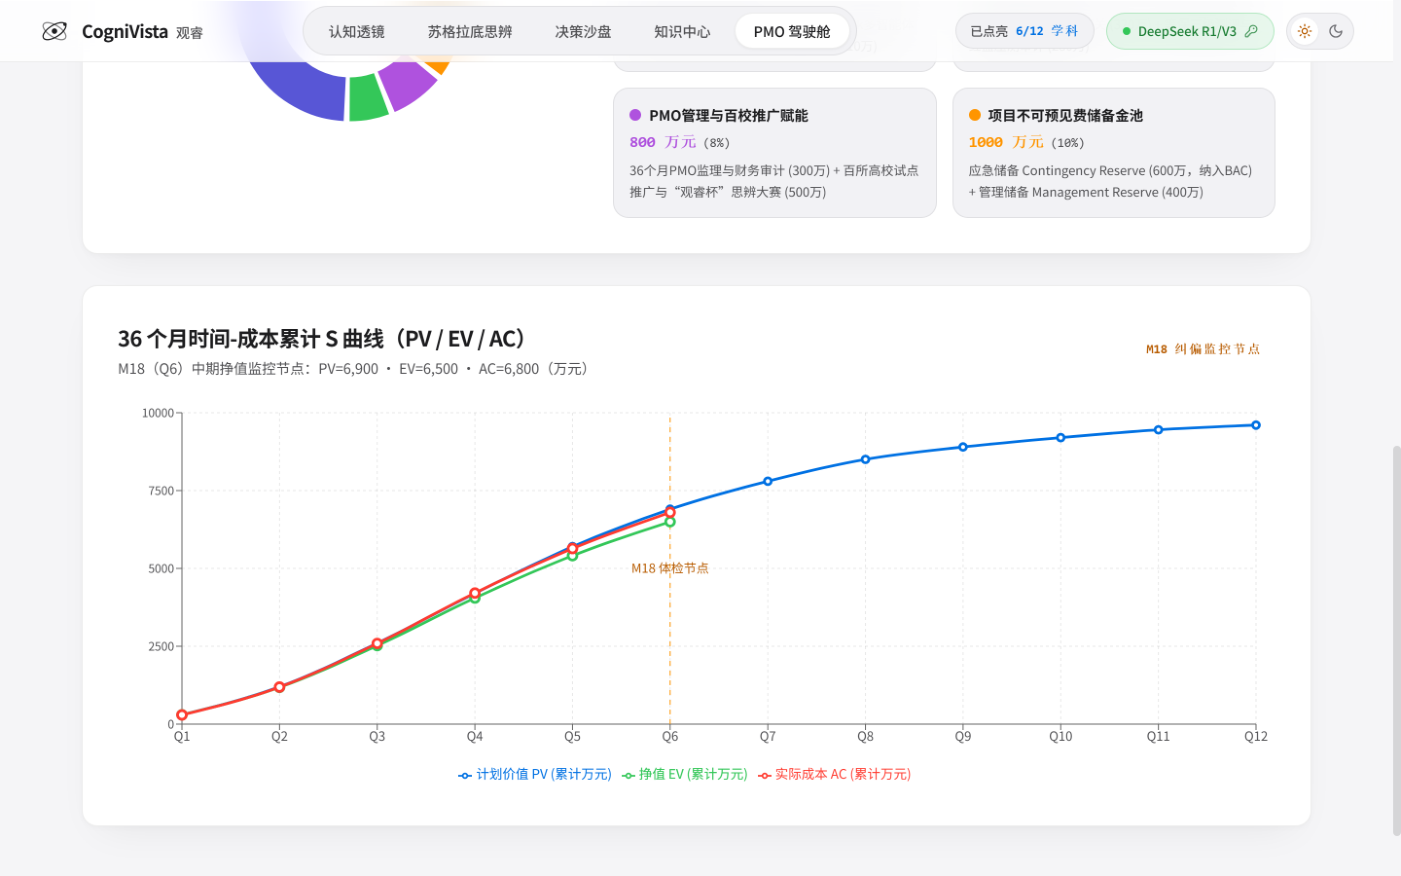
\includegraphics[width=0.82\linewidth,height=0.30\textheight,keepaspectratio]{figures/fig_06_pmo_cost_scurve.png}
    \caption{1 亿元预算结构与 36 个月资金使用计划}
    \label{fig:pmo_scurve}
\end{figure}

\subsection{中期挣值分析（EVM）与偏差纠偏}
挣值管理把费用和进度两条偏差放在一起看\textsuperscript{[6]}。本例假设 600 万元应急储备已经获批，转成了明确的风险应对工作预算，所以表~\ref{tab:evm} 只对已授权的任务计量挣值，没分配出去的储备不算挣值。第 18 个月，成本基准 9,600 万元，计划值 6,900 万元、挣值 6,500 万元、实际成本 6,800 万元。进度偏差是用预算金额表达的，不能直接换算成滞后几个月。

\begingroup
\linespread{1}\fontsize{9.5pt}{12pt}\selectfont\songti
\setlength{\tabcolsep}{3pt}
\renewcommand{\arraystretch}{1.18}
\begin{longtable}{@{}L{2.65cm}R{1.60cm}R{1.60cm}R{1.60cm}R{1.60cm}R{1.15cm}R{1.15cm}L{3.17cm}@{}}
\caption{M18 各账户挣值监控\label{tab:evm}} \\
\toprule[0.8pt]
\textbf{项目费用} & \textbf{BAC/万} & \textbf{PV/万} & \textbf{EV/万} & \textbf{AC/万} & \textbf{CPI} & \textbf{SPI} & \textbf{偏差说明} \\
\midrule[0.5pt]
\endfirsthead
\multicolumn{8}{@{}l@{}}{\linespread{1}\fontsize{9.5pt}{12pt}\selectfont\songti （续表）M18 各账户挣值监控} \\
\toprule[0.8pt]
\textbf{项目费用} & \textbf{BAC/万} & \textbf{PV/万} & \textbf{EV/万} & \textbf{AC/万} & \textbf{CPI} & \textbf{SPI} & \textbf{偏差说明} \\
\midrule[0.5pt]
\endhead
\bottomrule[0.8pt]
\endfoot
\bottomrule[0.8pt]
\endlastfoot
项目管理与推广 & 800.00 & 400.00 & 400.00 & 390.00 & 1.026 & 1.000 & 略有结余 \\
算力与网关 & 2,200.00 & 1,540.00 & 1,584.00 & 1,560.00 & 1.015 & 1.029 & 进度超前 \\
学科知识库 & 2,600.00 & 2,210.00 & 1,950.00 & 2,180.00 & 0.894 & 0.882 & 超支 230 万 \\
后端研发 & 1,400.00 & 1,120.00 & 1,092.00 & 1,130.00 & 0.966 & 0.975 & 轻微滞后 \\
前端研发 & 1,400.00 & 1,050.00 & 952.00 & 1,040.00 & 0.915 & 0.907 & 超支 88 万 \\
质量与安全 & 600.00 & 280.00 & 264.00 & 260.00 & 1.015 & 0.943 & 成本正常 \\
风险应对工作 & 600.00 & 300.00 & 258.00 & 240.00 & 1.075 & 0.860 & 执行中 \\
\midrule[0.4pt]
\textbf{M18 全项目总计} & \textbf{9,600.00} & \textbf{6,900.00} & \textbf{6,500.00} & \textbf{6,800.00} & \textbf{0.956} & \textbf{0.942} & \textbf{超支 300 万；进度偏差 400 万} \\
\end{longtable}
\endgroup

由这些数可以推出 M18 的核心绩效指标和完工尚需绩效指数（TCPI）：
\begin{equation}
\begin{aligned}
  \mathrm{CV} &= \mathrm{EV}-\mathrm{AC}=-300.00\text{ 万元},\\[4pt]
  \mathrm{SV} &= \mathrm{EV}-\mathrm{PV}=-400.00\text{ 万元}.
\end{aligned}
\end{equation}
\begin{equation}
\begin{aligned}
  \mathrm{CPI} &= \frac{6500}{6800}\approx 0.9559,\\[5pt]
  \mathrm{SPI} &= \frac{6500}{6900}\approx 0.9420,\\[5pt]
  \mathrm{TCPI}_{\mathrm{BAC}} &= \frac{9600-6500}{9600-6800}\approx 1.1071.
\end{aligned}
\end{equation}

拿还没四舍五入的绩效指数去预测完工估算（EAC）：假使剩余工作回到预算效率，$\mathrm{EAC}_1=\mathrm{AC}+(\mathrm{BAC}-\mathrm{EV})=9,900.00$ 万元，比成本基准高出 300 万元；假使当前的成本效率一直延续，$\mathrm{EAC}_2=\mathrm{BAC}/\mathrm{CPI}=10,043.08$ 万元；假使剩余工作同时被成本和进度效率两头拖累，$\mathrm{EAC}_3=\mathrm{AC}+(\mathrm{BAC}-\mathrm{EV})/(\mathrm{CPI}\times\mathrm{SPI})=10,242.65$ 万元。后两种情形都突破了总投资，在动用管理储备之前，得先把纠偏方案拿出来。

翻一下表~\ref{tab:evm} 就能看出，成本偏差主要出在知识库工程（超支 230 万元）和前端研发（超支 88 万元）两块。前者是公式文献解析返工闹的，后者是低配电脑渲染性能跟不上；其余账户的结余把超支抵消了一部分。

纠偏情景里排了三件事。其一，剩下 2,800 万页文献改成自动化解析，只留人工抽检：原单价 0.10 元/页，处理费降 45\% 能省 126 万元，扣掉部署和验证的 6 万元，净省 120 万元。其二，缓存之后剩余接口费用预计 720 万元，再优化一版按降 25\% 算，又能省 180 万元，原来那 35\% 的缓存比例不再重复扣。其三，从现有团队里抽 2 名图形开发人员支援两周，在原有人月预算内把分级渲染做完，不新增外包费用。

前两项加起来净省 300 万元，恢复预算效率情形下的完工估算就从 9,900 万元压回到 9,600 万元。假使采购结算和未发生的支出再省出 60 万元，模拟决算就是 9,540 万元，相对成本基准节余 60 万元，400 万元管理储备分文未动，总投资实际没花出去 460 万元。剩余工作的成本效率是 $3100\div 2740\approx 1.131$。不过上面这些节约和决算都是情景假设，得拿真实日志、合同和验收记录来验证。

\subsection{招采控本与成本变更分级审批}
招采文件里要把交付范围、验收标准、版权责任和退出条款写清楚，采购方式看资金性质和适用制度来定。合同付款跟交付验收绑在一起，试点没通过之前尾款不清，免得只顾按时间付钱。成本变更按影响大小分级：账户内调剂，项目经理审核备案即可；动应急储备，要过财务复核；改范围或基准，得上报 CCB 审议；管理储备由项目发起人批准。变更之后预算、进度、合同三本台账同步更新，别让审批和实际支出两张皮。

\section{项目质量、安全与资源管理}

\subsection{质量控制与 AI 安全伦理护栏}
质量管理要同时盯着软件交付和模型输出两头，生成内容的幻觉单独评\textsuperscript{[7]}。需求和设计阶段做同行评审，开发阶段把代码扫描和单元测试落到位，上线前再压测一遍。验收核对单列了五项指标：首字响应不超过 1.2 秒，检索召回率不低于 90\%，逻辑谬误识别准确率不低于 92\%，年可用性不低于 99.9\%，幻觉率不高于 1.5\%。这几个阈值是课程方案定的目标，得靠测试样本和场景去验证。

大模型应用要审查数据来源、偏见和误用风险\textsuperscript{[8]}。碰上直接代写的请求，就转成思路提示，回答必须绑上知识来源；幻觉率一旦超标，先停功能再排查。学生数据往外发之前要脱敏，权限按最小化配，访问留痕。试点前把安全测评和整改做完，高风险缺陷没关闭就不能上线。

\subsection{强矩阵组织与关键资源配置}
本项目用强矩阵组织：项目经理管预算、进度和交付统筹，专业负责人抓技术规范和人员培养，普通成员则要接受项目和专业两条线的协调。团队按管理、后端、知识库、前端、质量安全和推广运维六类职责来配。

专职人员一共 75 人，配置见表~\ref{tab:raci}；另外聘 120 名教师和博士生，覆盖 12 个学科门类，按任务包干语料标注和内容抽检。人员投入分阶段登记，防止同一个人月被重复计费。

表~\ref{tab:raci}《人力配置与责任矩阵》把执行（R）、唯一批准人（A）、咨询（C）、知会（I）四类职责标清楚。经理那一列含 1 名经理加 4 名项目管理办公室人员，批准责任由指定人员扛。人员错峰转岗，人月不能重复计费；20 台节点按需采购，文献走正规渠道授权。

\begingroup
\linespread{1}\fontsize{9pt}{11.5pt}\selectfont\songti
\setlength{\tabcolsep}{2.5pt}
\renewcommand{\arraystretch}{1.22}
\begin{longtable}{@{}L{4.27cm}C{1.50cm}C{1.50cm}C{1.50cm}C{1.50cm}C{1.50cm}C{1.50cm}C{1.50cm}@{}}
\caption{人力配置与责任矩阵\label{tab:raci}} \\
\toprule[0.8pt]
\textbf{核心管理与工程活动} & \textbf{项目经理} & \textbf{算力后端} & \textbf{知识工程} & \textbf{前端研发} & \textbf{质量安全} & \textbf{推广运维} & \textbf{学科顾问} \\
\midrule[0.5pt]
\endfirsthead
\multicolumn{8}{@{}l@{}}{\linespread{1}\fontsize{9pt}{11.5pt}\selectfont\songti （续表）人力配置与责任矩阵} \\
\toprule[0.8pt]
\textbf{核心管理与工程活动} & \textbf{项目经理} & \textbf{算力后端} & \textbf{知识工程} & \textbf{前端研发} & \textbf{质量安全} & \textbf{推广运维} & \textbf{学科顾问} \\
\midrule[0.5pt]
\endhead
\bottomrule[0.8pt]
\endfoot
\bottomrule[0.8pt]
\endlastfoot
团队人数（专职 75 人） & 经理 1 人\newline PMO 4 人 & 25 人 & 10 人 & 25 人 & 5 人 & 5 人 & 120 人 \\
\midrule[0.4pt]
范围及预算基准与挣值纠偏 & A/R & C & C & C & I & I & I \\
DeepSeek 网关与缓存建设 & A & R & C & I & C & I & I \\
12 学科文献清洗与标注 & A & I & R & I & C & I & R/C \\
四类交互功能与多端适配 & A & C & I & R & C & I & C \\
安全测评与内容质量审核 & A & C & C & C & R & I & C \\
百校推广、大赛与运维验收 & A & I & I & I & I & R & C \\
\end{longtable}
\endgroup

\section{项目风险管理}

\subsection{风险识别与 EMV 定量储备测算}
风险管理得贴着项目技术上的不确定性，持续做识别、分析和应对\textsuperscript{[9]}。本方案覆盖接口、内容、版权、性能、留存和数据安全六类风险，概率和损失按月复核。表里的概率都是课程情景假设，用期望损失来估储备规模：
\begin{equation}
  \mathrm{EMV}_{\mathrm{total}} = \sum_{k=1}^{6} (P_k \times I_k) = 592.00\text{ 万元}
\end{equation}
592 万元只是期望损失，不打包票能覆盖最坏情形。初始储备要过相关性和情景压力测试这关，转成任务预算后就不能再当作可用储备重复列了。

\subsection{核心风险登记册与应对预案}
表~\ref{tab:risk}《风险测算与应对计划》里的概率和损失都是课程假设，不是调研统计出来的。风险登记册按月更新，事件发生后由责任人记下处置成本，回头复核剩余风险和储备，审批与关闭的记录都要留好。

\begingroup
\linespread{1}\fontsize{9.5pt}{12pt}\selectfont\songti
\setlength{\tabcolsep}{3.5pt}
\renewcommand{\arraystretch}{1.18}
\begin{longtable}{@{}L{4.00cm}C{0.95cm}R{1.50cm}R{1.45cm}L{2.25cm}L{4.61cm}@{}}
\caption{风险测算与应对计划\label{tab:risk}} \\
\toprule[0.8pt]
\textbf{风险事件} & \textbf{概率} & \textbf{损失/万} & \textbf{EMV/万} & \textbf{策略及责任人} & \textbf{预防与应急措施} \\
\midrule[0.5pt]
\endfirsthead
\multicolumn{6}{@{}l@{}}{\linespread{1}\fontsize{9.5pt}{12pt}\selectfont\songti （续表）风险测算与应对计划} \\
\toprule[0.8pt]
\textbf{风险事件} & \textbf{概率} & \textbf{损失/万} & \textbf{EMV/万} & \textbf{策略及责任人} & \textbf{预防与应急措施} \\
\midrule[0.5pt]
\endhead
\bottomrule[0.8pt]
\endfoot
\bottomrule[0.8pt]
\endlastfoot
期末高峰 API 限流或中断 & 25\% & 480.00 & 120.00 & 减轻、转移\newline 架构师 & 设置缓存与备用通道；异常时限流降级、告警并切换服务，定期演练恢复。 \\
跨学科议题幻觉超标 & 30\% & 400.00 & 120.00 & 减轻、规避\newline 质量负责人 & 回答强制溯源并抽检；幻觉率超标时暂停相关功能，修复后复测。 \\
文献清洗返工与版权纠纷 & 20\% & 700.00 & 140.00 & 规避、转移\newline 知识负责人 & 清洗先抽检，版权先核验；争议内容暂停访问，返工重估工时。 \\
星系图在低配本掉帧 & 35\% & 240.00 & 84.00 & 减轻\newline 前端负责人 & 采用分级渲染与卡片模式；目标设备帧率不足时减少图谱节点。 \\
学习负担增加、留存下降 & 25\% & 320.00 & 80.00 & 减轻\newline 项目经理 & 以自愿试点和学习反馈改进引导；留存下降时访谈诊断，不以强制考核替代效果验证。 \\
学生隐私泄露或渗透攻击 & 16\% & 300.00 & 48.00 & 规避、减轻\newline 安全负责人 & 请求分类脱敏、最小权限与审计；异常外发时暂停接口并排查，不把实体识别当作充分匿名化。 \\
\midrule[0.4pt]
\textbf{风险期望损失合计} & \textbf{—} & \textbf{2,440.00} & \textbf{592.00} & \textbf{—} & \textbf{初始预留 600 万元应急储备。} \\
\end{longtable}
\endgroup

\section{项目后评价与工程管理总结}

\subsection{竣工决算与多维后评价}
后评价不该只停在工期和成本上，还要看交付价值和服务效果\textsuperscript{[10]}。表~\ref{tab:post} 是第 36 个月的模拟核查，不算真实验收。工期 35.5 个月、覆盖 118 校 135 万人、决算 9,540 万元，这些数字都只用来演示评价方法。真要实施，交付和财务记录得核验；学习成效用前后测加对照组比较，运营收支另按续费和运维费用去测。

\begingroup
\linespread{1}\fontsize{9.5pt}{12pt}\selectfont\songti
\setlength{\tabcolsep}{3.5pt}
\renewcommand{\arraystretch}{1.20}
\begin{longtable}{@{}L{1.60cm}L{2.95cm}L{2.95cm}L{3.35cm}L{4.16cm}@{}}
\caption{竣工决算与后评价\label{tab:post}} \\
\toprule[0.8pt]
\textbf{评价维度} & \textbf{核心指标} & \textbf{立项目标} & \textbf{模拟结果或评价方法} & \textbf{评价要点} \\
\midrule[0.5pt]
\endfirsthead
\multicolumn{5}{@{}l@{}}{\linespread{1}\fontsize{9.5pt}{12pt}\selectfont\songti （续表）竣工决算与后评价} \\
\toprule[0.8pt]
\textbf{评价维度} & \textbf{核心指标} & \textbf{立项目标} & \textbf{模拟结果或评价方法} & \textbf{评价要点} \\
\midrule[0.5pt]
\endhead
\bottomrule[0.8pt]
\endfoot
\bottomrule[0.8pt]
\endlastfoot
过程评价 & 总工期与决算成本 & 36 个月；成本基准 9,600 万元 & 模拟 35.5 个月；决算 9,540 万元 & 较基准节余 60 万元；管理储备 400 万元未用 \\
过程评价 & 范围与 AI 质量验收 & 安全测评；幻觉率不高于 1.5\% & 按验收与抽检报告复核 & 核查功能交付、测试样本与缺陷关闭记录 \\
服务效能 & 高校与学生覆盖 & 100 校；100 万人 & 模拟覆盖 118 校、135 万人 & 核对去重用户与有效使用记录，区分注册和活跃人数 \\
认知成效 & 跨学科与思辨能力 & 建立可重复的测评方法 & 采用前后测与对照组比较 & 控制原有能力差异，报告样本、指标和局限 \\
可持续性 & 建设期后运营机制 & 测算运营收支 & 会费与续费收入；运维支出测算 & 按续费率与运维费用核算，不预先认定自平衡 \\
\end{longtable}
\endgroup

\subsection{工程管理总结}
本报告是 36 个月、1 亿元平台建设的课程模拟方案。从预算推演和管理安排里能归纳出几条经验，但不能据此说项目已经建成、或者拿到了实测收益。

头一条，选技术要比较全生命周期成本。本方案把知识库和交互研发当主要投入，后续支出则靠接口替换、缓存和资源回收压着。外部模型服务本身也有涨价和供应中断的风险，不能只盯着初期的采购价。

再一条，预算控制得把交付任务、成本科目和时间基准对上号，按月比计划值、挣值和实际成本。一有偏差，先查返工和资源效率，再决定是调方案还是申请储备，审批和复核的记录要留全。

最后一条，教育平台验收既查性能、安全和版权，也要靠独立测评看学习效果。课程模拟里预算平衡、进度达标，只能说明管理方案算得通，实际成效还得在试点里验，再根据结果调整推广的规模。

% ---------- 参考文献（整组另起一页） ----------
\clearpage
\begin{thebibliography}{10}
\bibitem{ref1} ZAWACKI-RICHTER O, MAR\'IN V I, BOND M, et al. Systematic review of research on artificial intelligence applications in higher education -- where are the educators?[J]. International Journal of Educational Technology in Higher Education, 2019, 16: 39.
\bibitem{ref2} KASNECI E, SESSLER K, K\"UCHEMANN S, et al. ChatGPT for good? On opportunities and challenges of large language models for education[J]. Learning and Individual Differences, 2023, 103: 102274.
\bibitem{ref3} GUO D, YANG D, ZHANG H, et al. DeepSeek-R1 incentivizes reasoning in LLMs through reinforcement learning[J]. Nature, 2025, 645(8081): 633-638.
\bibitem{ref4} LEWIS P, PEREZ E, PIKTUS A, et al. Retrieval-Augmented Generation for Knowledge-Intensive NLP Tasks[C]//Advances in Neural Information Processing Systems. Red Hook: Curran Associates, 2020, 33: 9459-9474.
\bibitem{ref5} FLYVBJERG B, HOLM M S, BUHL S. Underestimating costs in public works projects: Error or lie?[J]. Journal of the American Planning Association, 2002, 68(3): 279-295.
\bibitem{ref6} VANDEVOORDE S, VANHOUCKE M. A comparison of different project duration forecasting methods using earned value metrics[J]. International Journal of Project Management, 2006, 24(4): 289-302.
\bibitem{ref7} JI Z, LEE N, FRIESKE R, et al. Survey of hallucination in natural language generation[J]. ACM Computing Surveys, 2023, 55(12): Article 248, 1-38.
\bibitem{ref8} BENDER E M, GEBRU T, MCMILLAN-MAJOR A, et al. On the dangers of stochastic parrots: Can language models be too big?[C]//Proceedings of the 2021 ACM Conference on Fairness, Accountability, and Transparency. New York: ACM, 2021: 610-623.
\bibitem{ref9} RAZ T, SHENHAR A J, DVIR D. Risk management, project success, and technological uncertainty[J]. R\&D Management, 2002, 32(2): 101-109.
\bibitem{ref10} ATKINSON R. Project management: Cost, time and quality, two best guesses and a phenomenon, its time to accept other success criteria[J]. International Journal of Project Management, 1999, 17(6): 337-342.
\end{thebibliography}

\end{document}
